%----------------------------------------------------------------------------
%----------------------------------------------------------------------------
First, the raw data sets are calibrated. The computer records the voltage sampled from the SR250 verses the associated voltage level sent to the receiver from the voltage ramp. The relationship between voltage sent to the receiver and the corresponding center frequency of the receiver is obtained by taking pictures of the laptop computer next to the HP 53132A counter. Each picture shows the current voltage on the voltage ramp (displayed on the laptop screen) and the current center frequency of the receiver. Several such pictures are taken during each scan. The relationship is found to be very linear, but shifts a little bit from scan to scan.

Once calibrated, each scan is scaled to compensate for the response curve of the photodiode (see AHI02-DN3300-5-VR08). Only one of the two photodiodes was calibrated (S/N 878) - here we use the one that wasn't calibrated and assume it has a similar response. See Figs. \ref{22-12}
%----------------------------------------------------------------------------
%----------------------------------------------------------------------------
%bb defines the bounding box for the pdf
%viewport defines the area of the pdf used
%in sidewaysfigure the last entry in bb moves the caption toward/away the pic
%in sidewaysfigure the second entry in bb moves the pic toward/away the caption
%----------------------------------------------------------------------------
\begin{figure}
\scalebox{0.8}[0.6]{
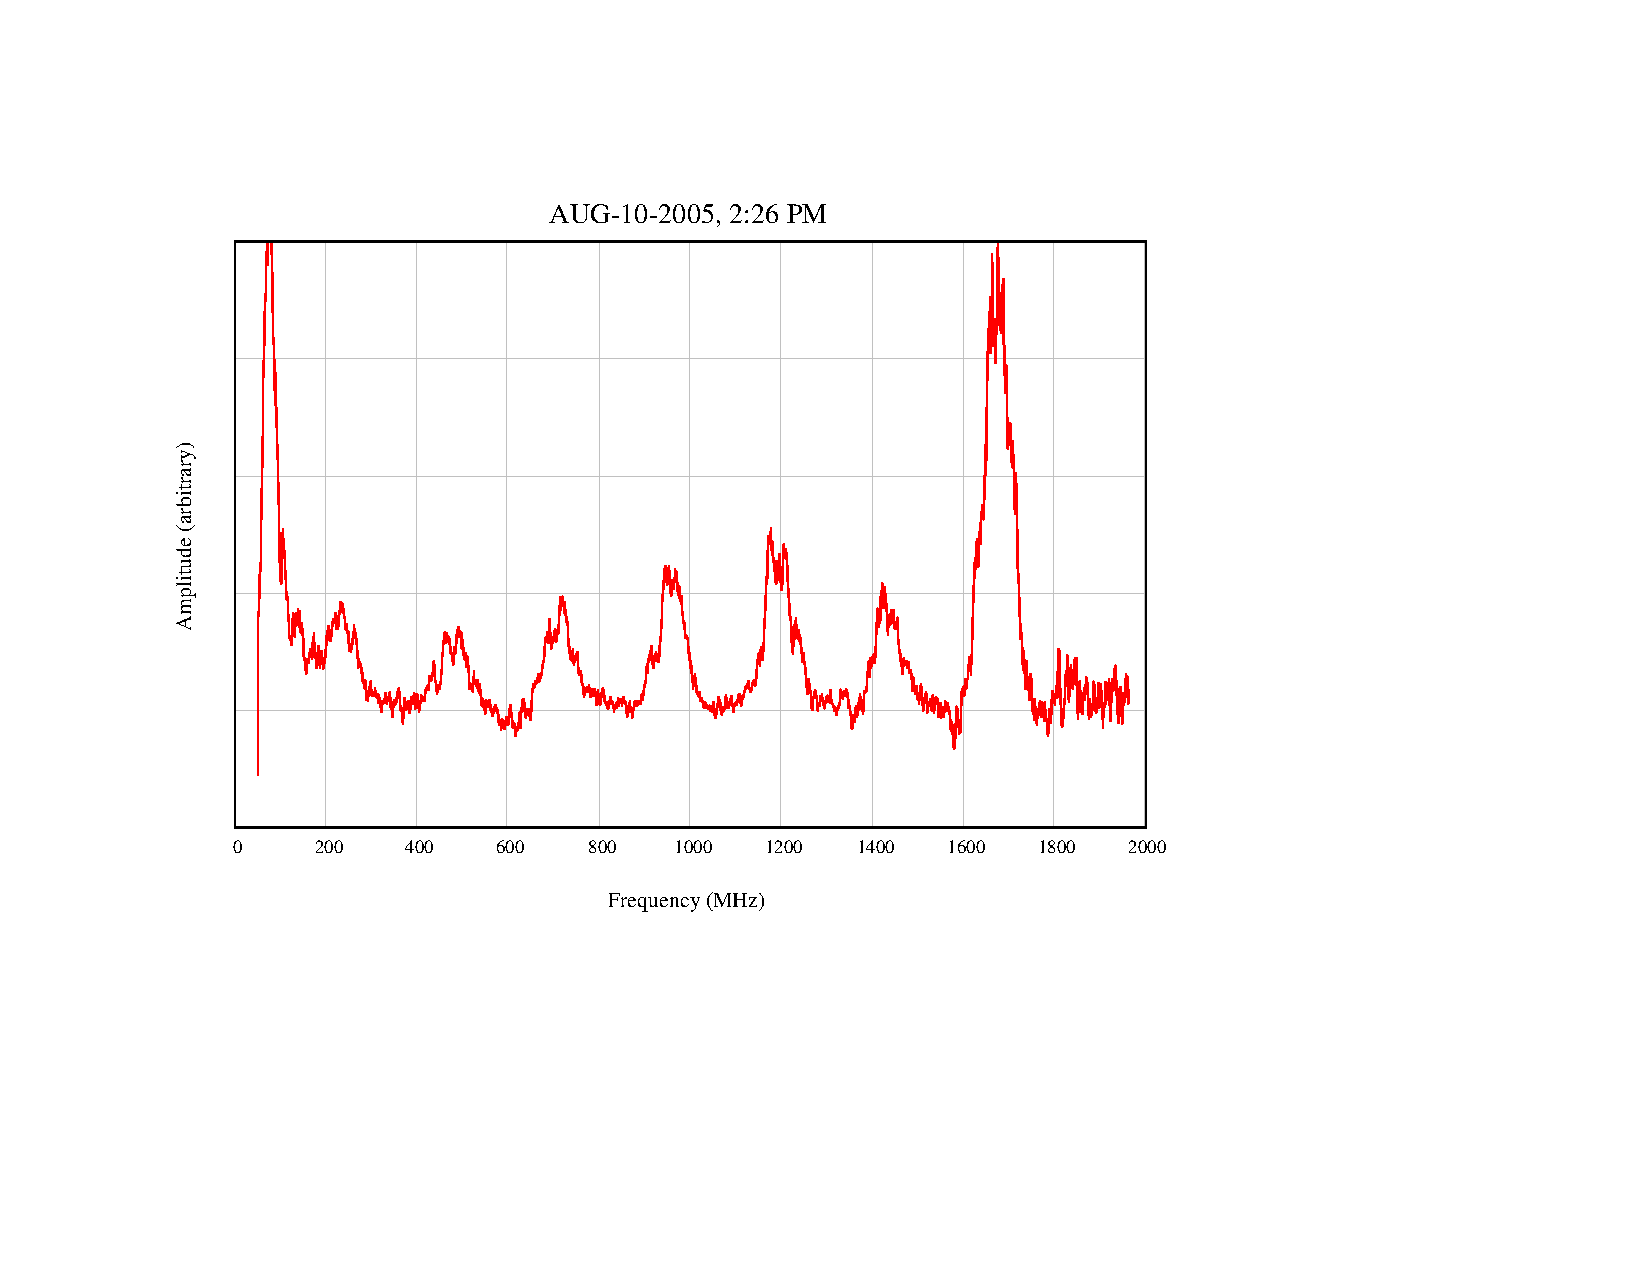
\includegraphics[viewport=150 200 300 450, bb=85 160 300 550]
{22-12/22-12.pdf}
}
\caption{Dye laser \#22 scanned with the 7L12}
\label{22-12}
\end{figure}
%----------------------------------------------------------------------------

%----------------------------------------------------------------------------
and \ref{22-14}
%----------------------------------------------------------------------------
%----------------------------------------------------------------------------
%bb defines the bounding box for the pdf
%viewport defines the area of the pdf used
%in sidewaysfigure the last entry in bb moves the caption toward/away the pic
%in sidewaysfigure the second entry in bb moves the pic toward/away the caption
%----------------------------------------------------------------------------
\begin{figure}
\scalebox{0.8}[0.6]{
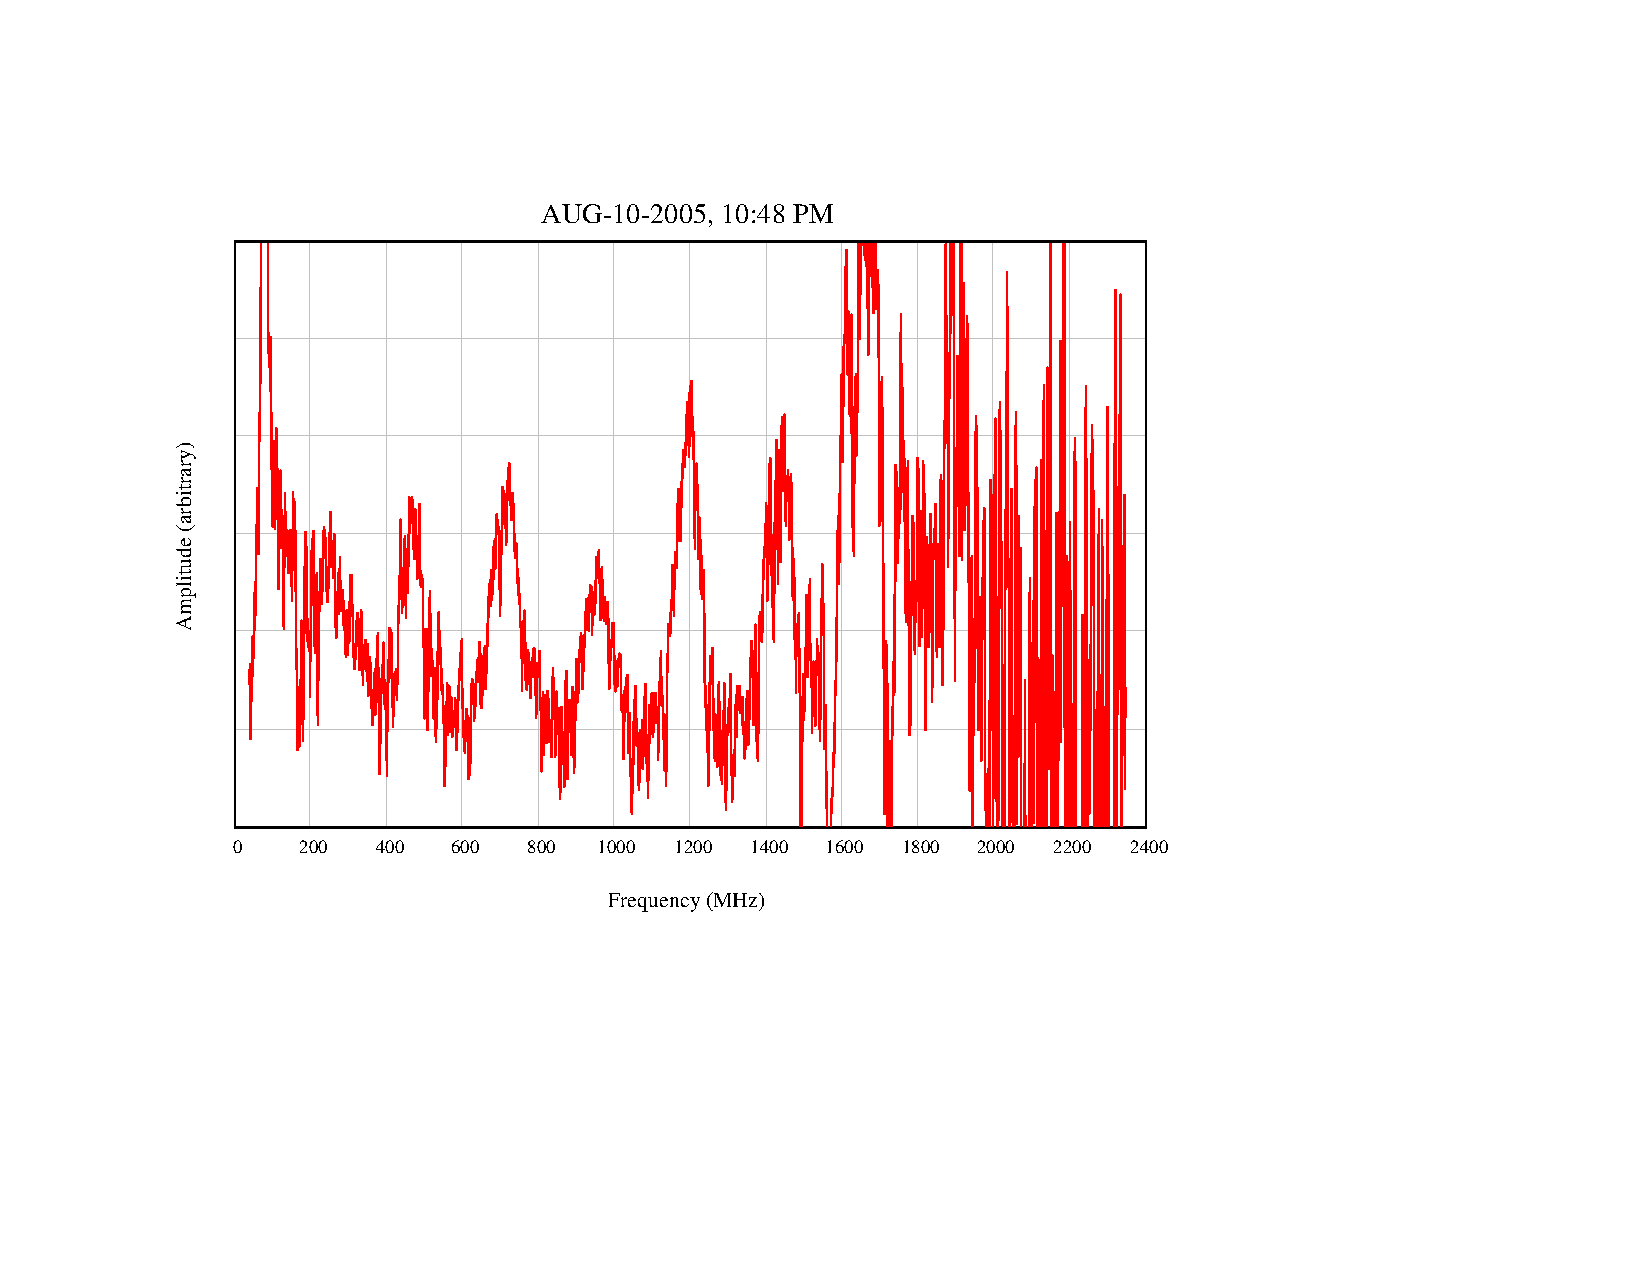
\includegraphics[viewport=150 200 300 450, bb=85 160 300 550]
{22-14/22-14.pdf}
}
\caption{Dye laser \#22 scanned with the 7L14}
\label{22-14}
\end{figure}
%----------------------------------------------------------------------------

%----------------------------------------------------------------------------
to see the data for dye laser \#22 taken with the 7L12 and 7L14 respectively. See Figs. \ref{23-12}
%----------------------------------------------------------------------------
%----------------------------------------------------------------------------
%bb defines the bounding box for the pdf
%viewport defines the area of the pdf used
%in sidewaysfigure the last entry in bb moves the caption toward/away the pic
%in sidewaysfigure the second entry in bb moves the pic toward/away the caption
%----------------------------------------------------------------------------
\begin{figure}
\scalebox{0.8}[0.6]{
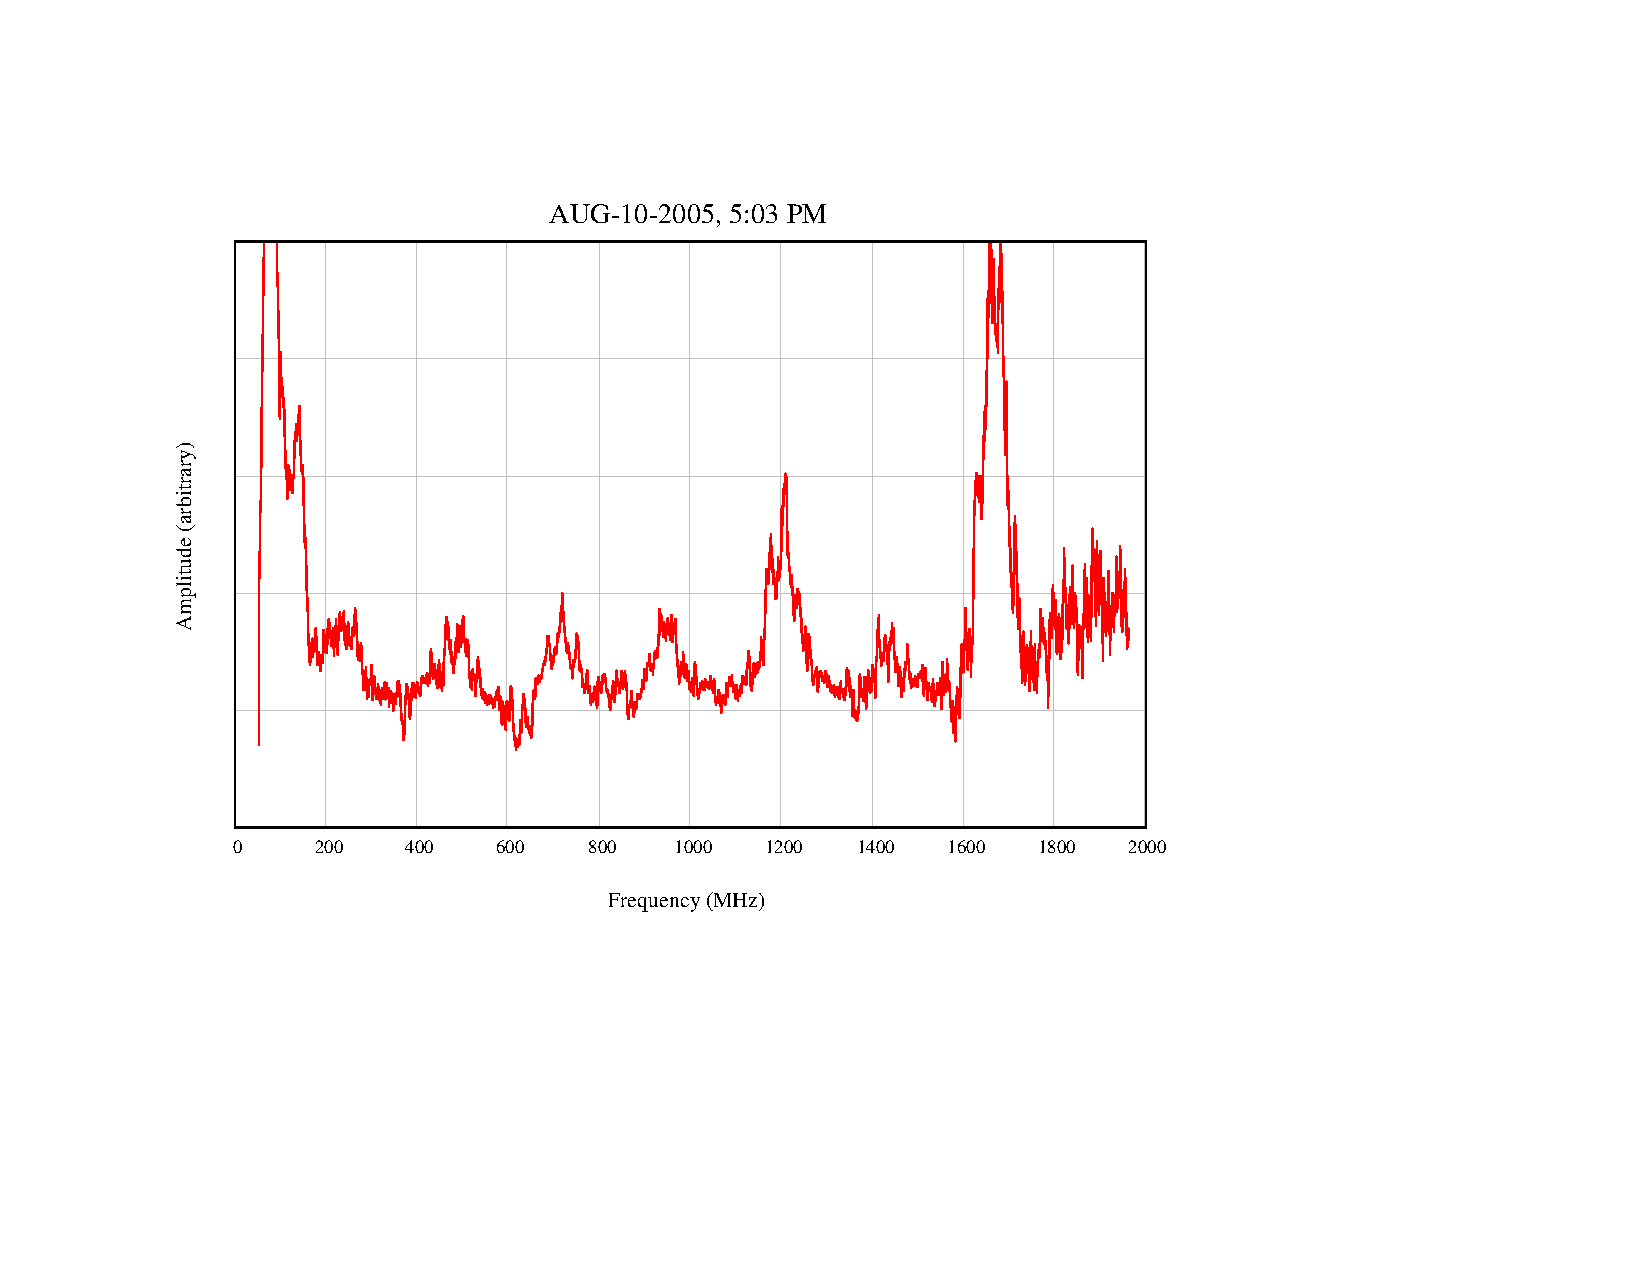
\includegraphics[viewport=150 200 300 450, bb=85 160 300 550]
{23-12/23-12.pdf}
}
\caption{Dye laser \#23 scanned with the 7L12}
\label{23-12}
\end{figure}
%----------------------------------------------------------------------------

%----------------------------------------------------------------------------
and \ref{23-14}
%----------------------------------------------------------------------------
%----------------------------------------------------------------------------
%bb defines the bounding box for the pdf
%viewport defines the area of the pdf used
%in sidewaysfigure the last entry in bb moves the caption toward/away the pic
%in sidewaysfigure the second entry in bb moves the pic toward/away the caption
%----------------------------------------------------------------------------
\begin{figure}
\scalebox{0.8}[0.6]{
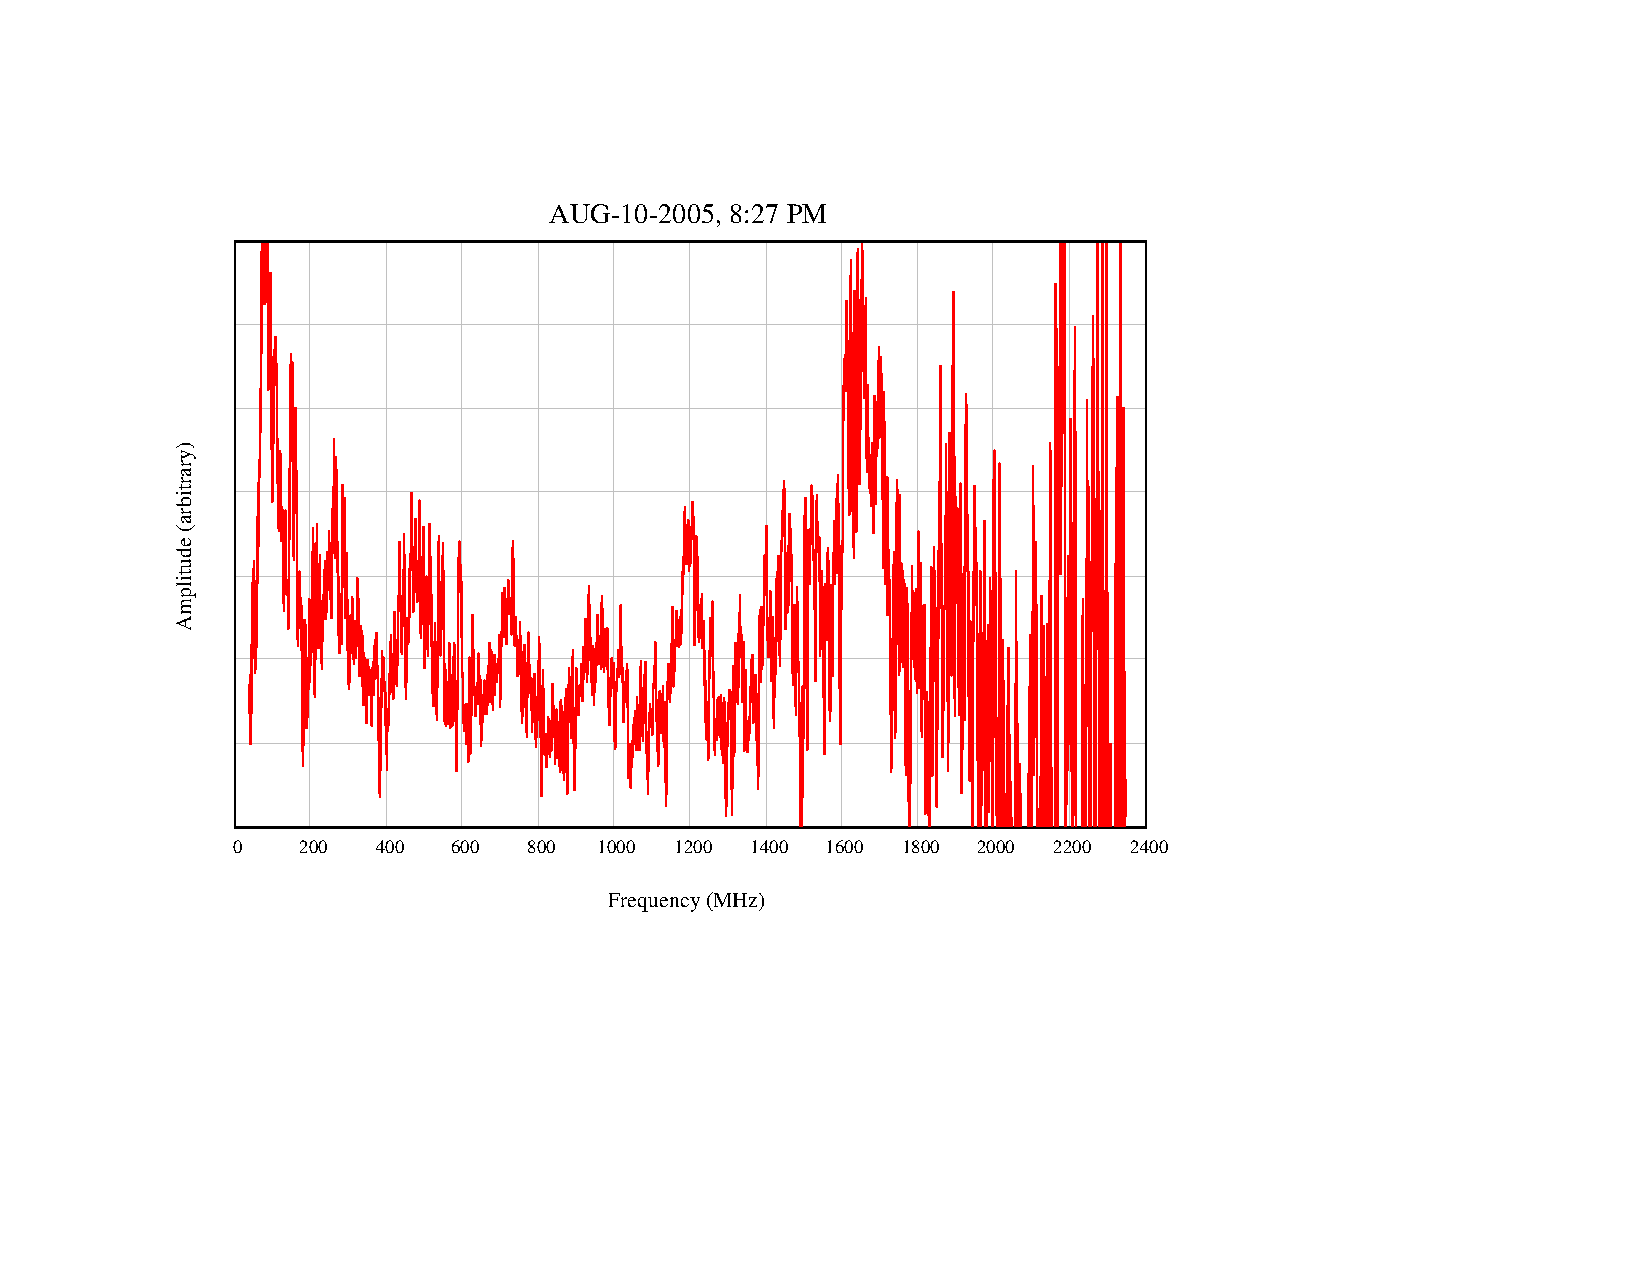
\includegraphics[viewport=150 200 300 450, bb=85 160 300 550]
{23-14/23-14.pdf}
}
\caption{Dye laser \#23 scanned with the 7L14}
\label{23-14}
\end{figure}
%----------------------------------------------------------------------------

%----------------------------------------------------------------------------
to see the data for dye laser \#23 taken with the 7L12 and 7L14 respectively. The following overlays are of the raw data - calibrated but not scaled for the photodiode response. Figs. \ref{2X-12}
%----------------------------------------------------------------------------
%----------------------------------------------------------------------------
%bb defines the bounding box for the pdf
%viewport defines the area of the pdf used
%in sidewaysfigure the last entry in bb moves the caption toward/away the pic
%in sidewaysfigure the second entry in bb moves the pic toward/away the caption
%----------------------------------------------------------------------------
\begin{figure}
\scalebox{0.8}[0.6]{
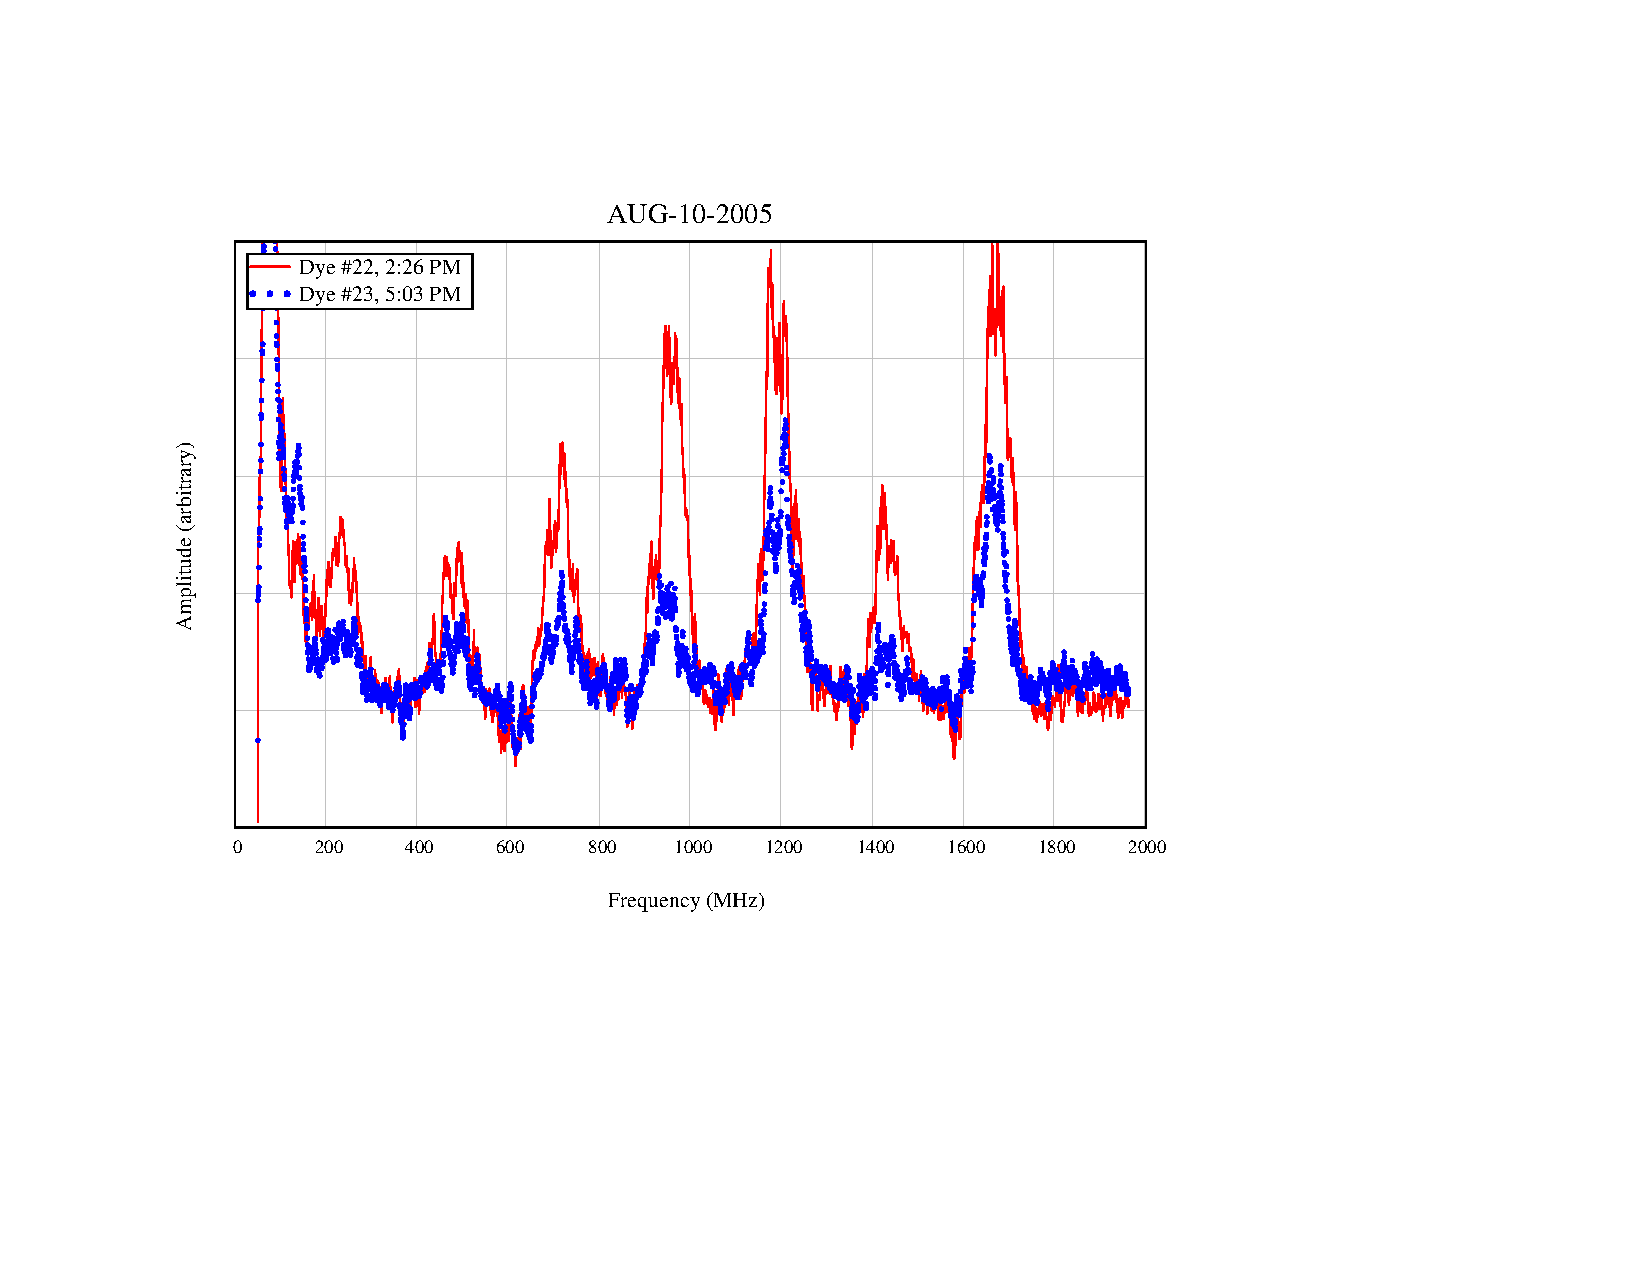
\includegraphics[viewport=150 200 300 450, bb=85 160 300 550]
{2X-12/2X-12.pdf}
}
\caption{Both dye lasers scanned with the 7L12 (raw data)}
\label{2X-12}
\end{figure}
%----------------------------------------------------------------------------

%----------------------------------------------------------------------------
and \ref{2X-14}
%----------------------------------------------------------------------------
%----------------------------------------------------------------------------
%bb defines the bounding box for the pdf
%viewport defines the area of the pdf used
%in sidewaysfigure the last entry in bb moves the caption toward/away the pic
%in sidewaysfigure the second entry in bb moves the pic toward/away the caption
%----------------------------------------------------------------------------
\begin{figure}
\scalebox{0.8}[0.6]{
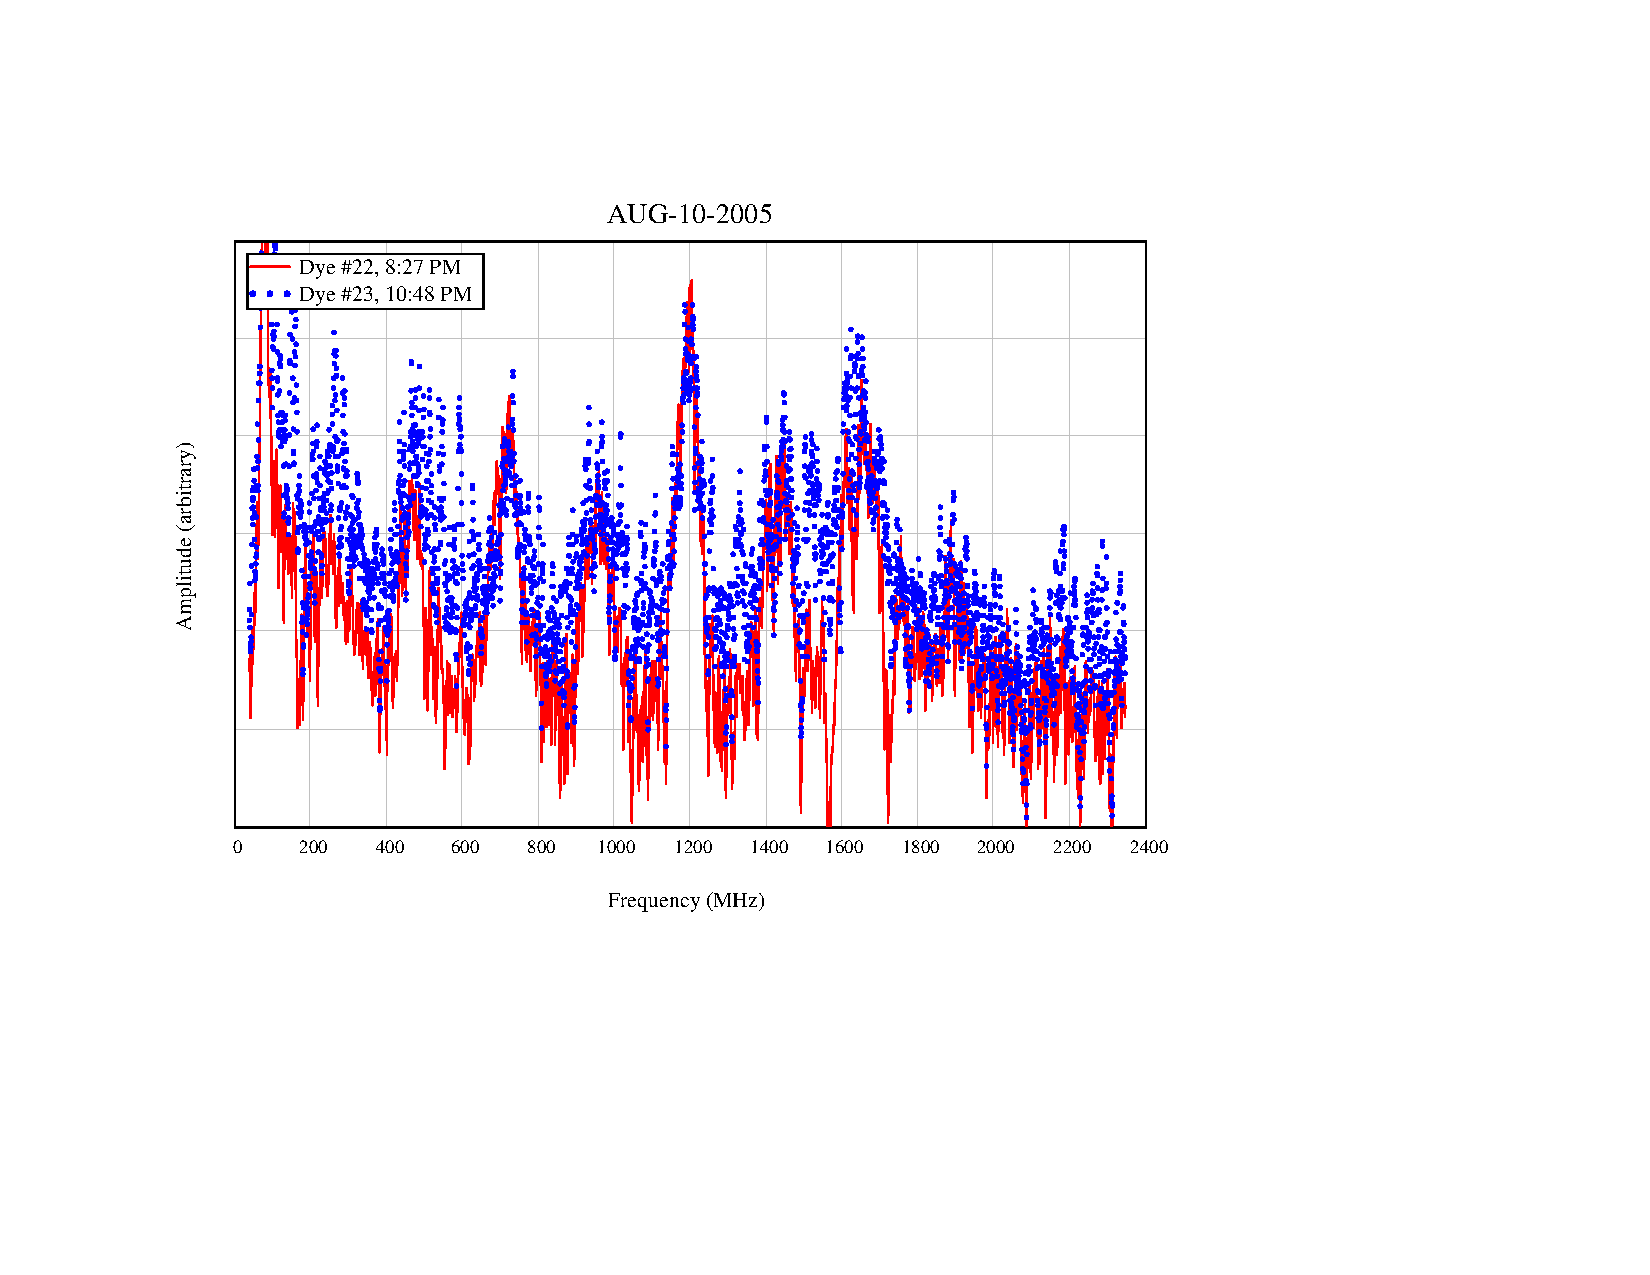
\includegraphics[viewport=150 200 300 450, bb=85 160 300 550]
{2X-14/2X-14.pdf}
}
\caption{Both dye lasers scanned with the 7L14 (raw data)}
\label{2X-14}
\end{figure}
%----------------------------------------------------------------------------

%----------------------------------------------------------------------------
show overlays of the data from the two lasers taken with the 7L12 and 7L14 respectively. Fig. \ref{23-12-seederX}
%----------------------------------------------------------------------------
%----------------------------------------------------------------------------
%bb defines the bounding box for the pdf
%viewport defines the area of the pdf used
%in sidewaysfigure the last entry in bb moves the caption toward/away the pic
%in sidewaysfigure the second entry in bb moves the pic toward/away the caption
%----------------------------------------------------------------------------
\begin{figure}
\scalebox{0.8}[0.6]{
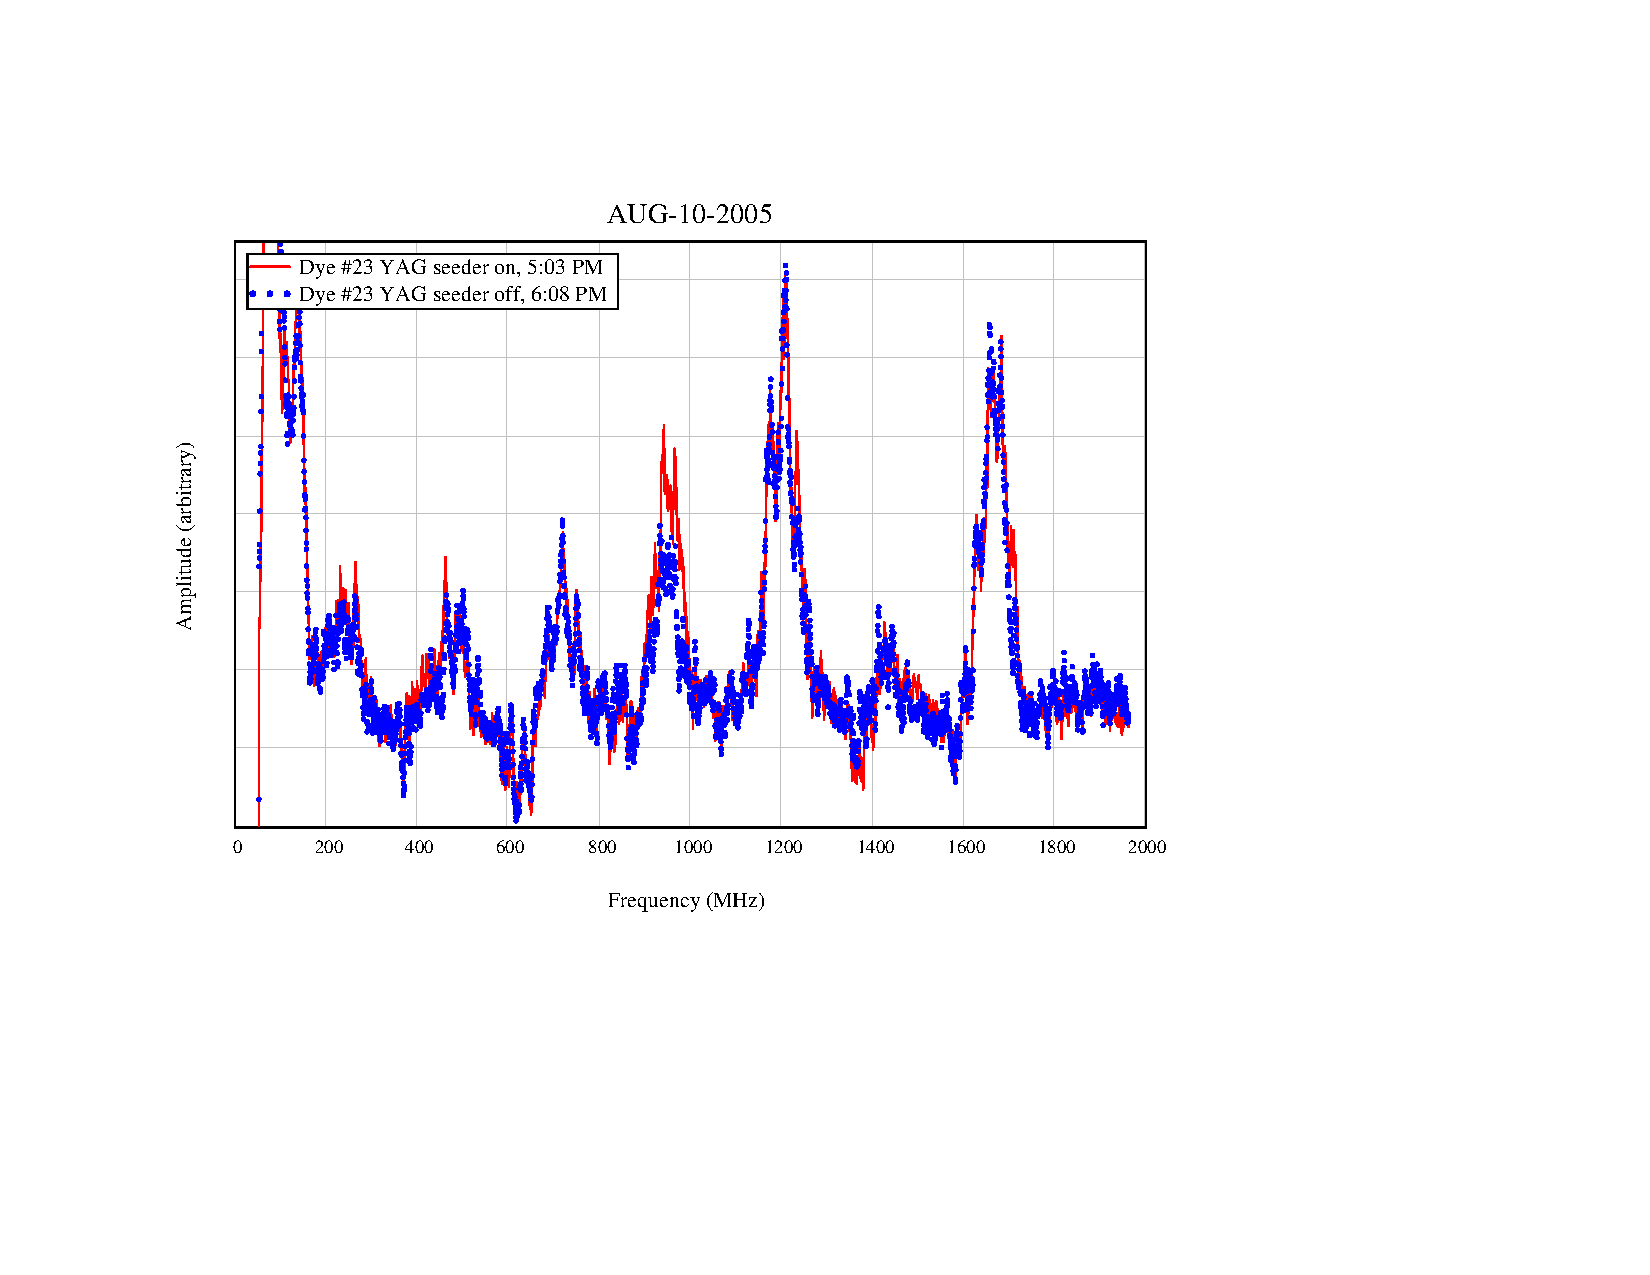
\includegraphics[viewport=150 200 300 450, bb=85 160 300 550]
{23-12-seederX/23-12-seederX.pdf}
}
\caption{Dye laser \# 23, with YAG pump with the seeder on/off, scanned with the 7L12 (raw data)}
\label{23-12-seederX}
\end{figure}
%----------------------------------------------------------------------------

%----------------------------------------------------------------------------
shows an overlay of the data from dye laser \#23 with the YAG pump in two states: seeder on and seeder off.

Finally, to check the spectral width of the observed features, the peak at 1200 MHz from the 7L12 scan of the \#23 dye laser is fit to a Gaussian (see Fig. \ref{fit}).
%----------------------------------------------------------------------------
%----------------------------------------------------------------------------
%bb defines the bounding box for the pdf
%viewport defines the area of the pdf used
%in sidewaysfigure the last entry in bb moves the caption toward/away the pic
%in sidewaysfigure the second entry in bb moves the pic toward/away the caption
%----------------------------------------------------------------------------
\begin{figure}
\scalebox{0.7}[0.7]{
\includegraphics*[bb=75 286 643 540]
{fit/fit.pdf}
}
\caption[Gaussinan fit for a single RF beat spectral feature]{The spectral feature at 1200 MHz fits a Gaussian with a FWHM of 83 MHz. This corresponds to a Gaussian in the time domain with a FWHM of 7.5 ns. This matches the observed pulse width - implying each mode is transform limited.}
\label{fit}
\end{figure}
%----------------------------------------------------------------------------

%----------------------------------------------------------------------------
Using the FWHM from the fit, Eqn. \ref{receiver width} is used to determine the corresponding transform limited temporal width.
%----------------------------------------------------------------------------
%----------------------------------------------------------------------------
